\subsection{RQ2: Which implementation technologies and tools are adopted by software development professionals?}
\label{RQ2}
The answer of this question covers a large area. To answer the question fully, we report the following results:
\begin{itemize}
\item Technology Platform (Q 9).
\item Operating System (Q 10).
\item Programming Language (Q 11).
\item Framework (Q 12).
\item IDE (Q 13).
\end{itemize}

\subsubsection{Technology Platforms}
Participants were allowed to choose multiple option. As shown in \cref{fig:platforms}, most of the respondents worked in web platform (47\%). The rests were mobile (28\%), Desktop (18\%), Embedded/IOT (5\%).
\begin{figure}[]
\centering
  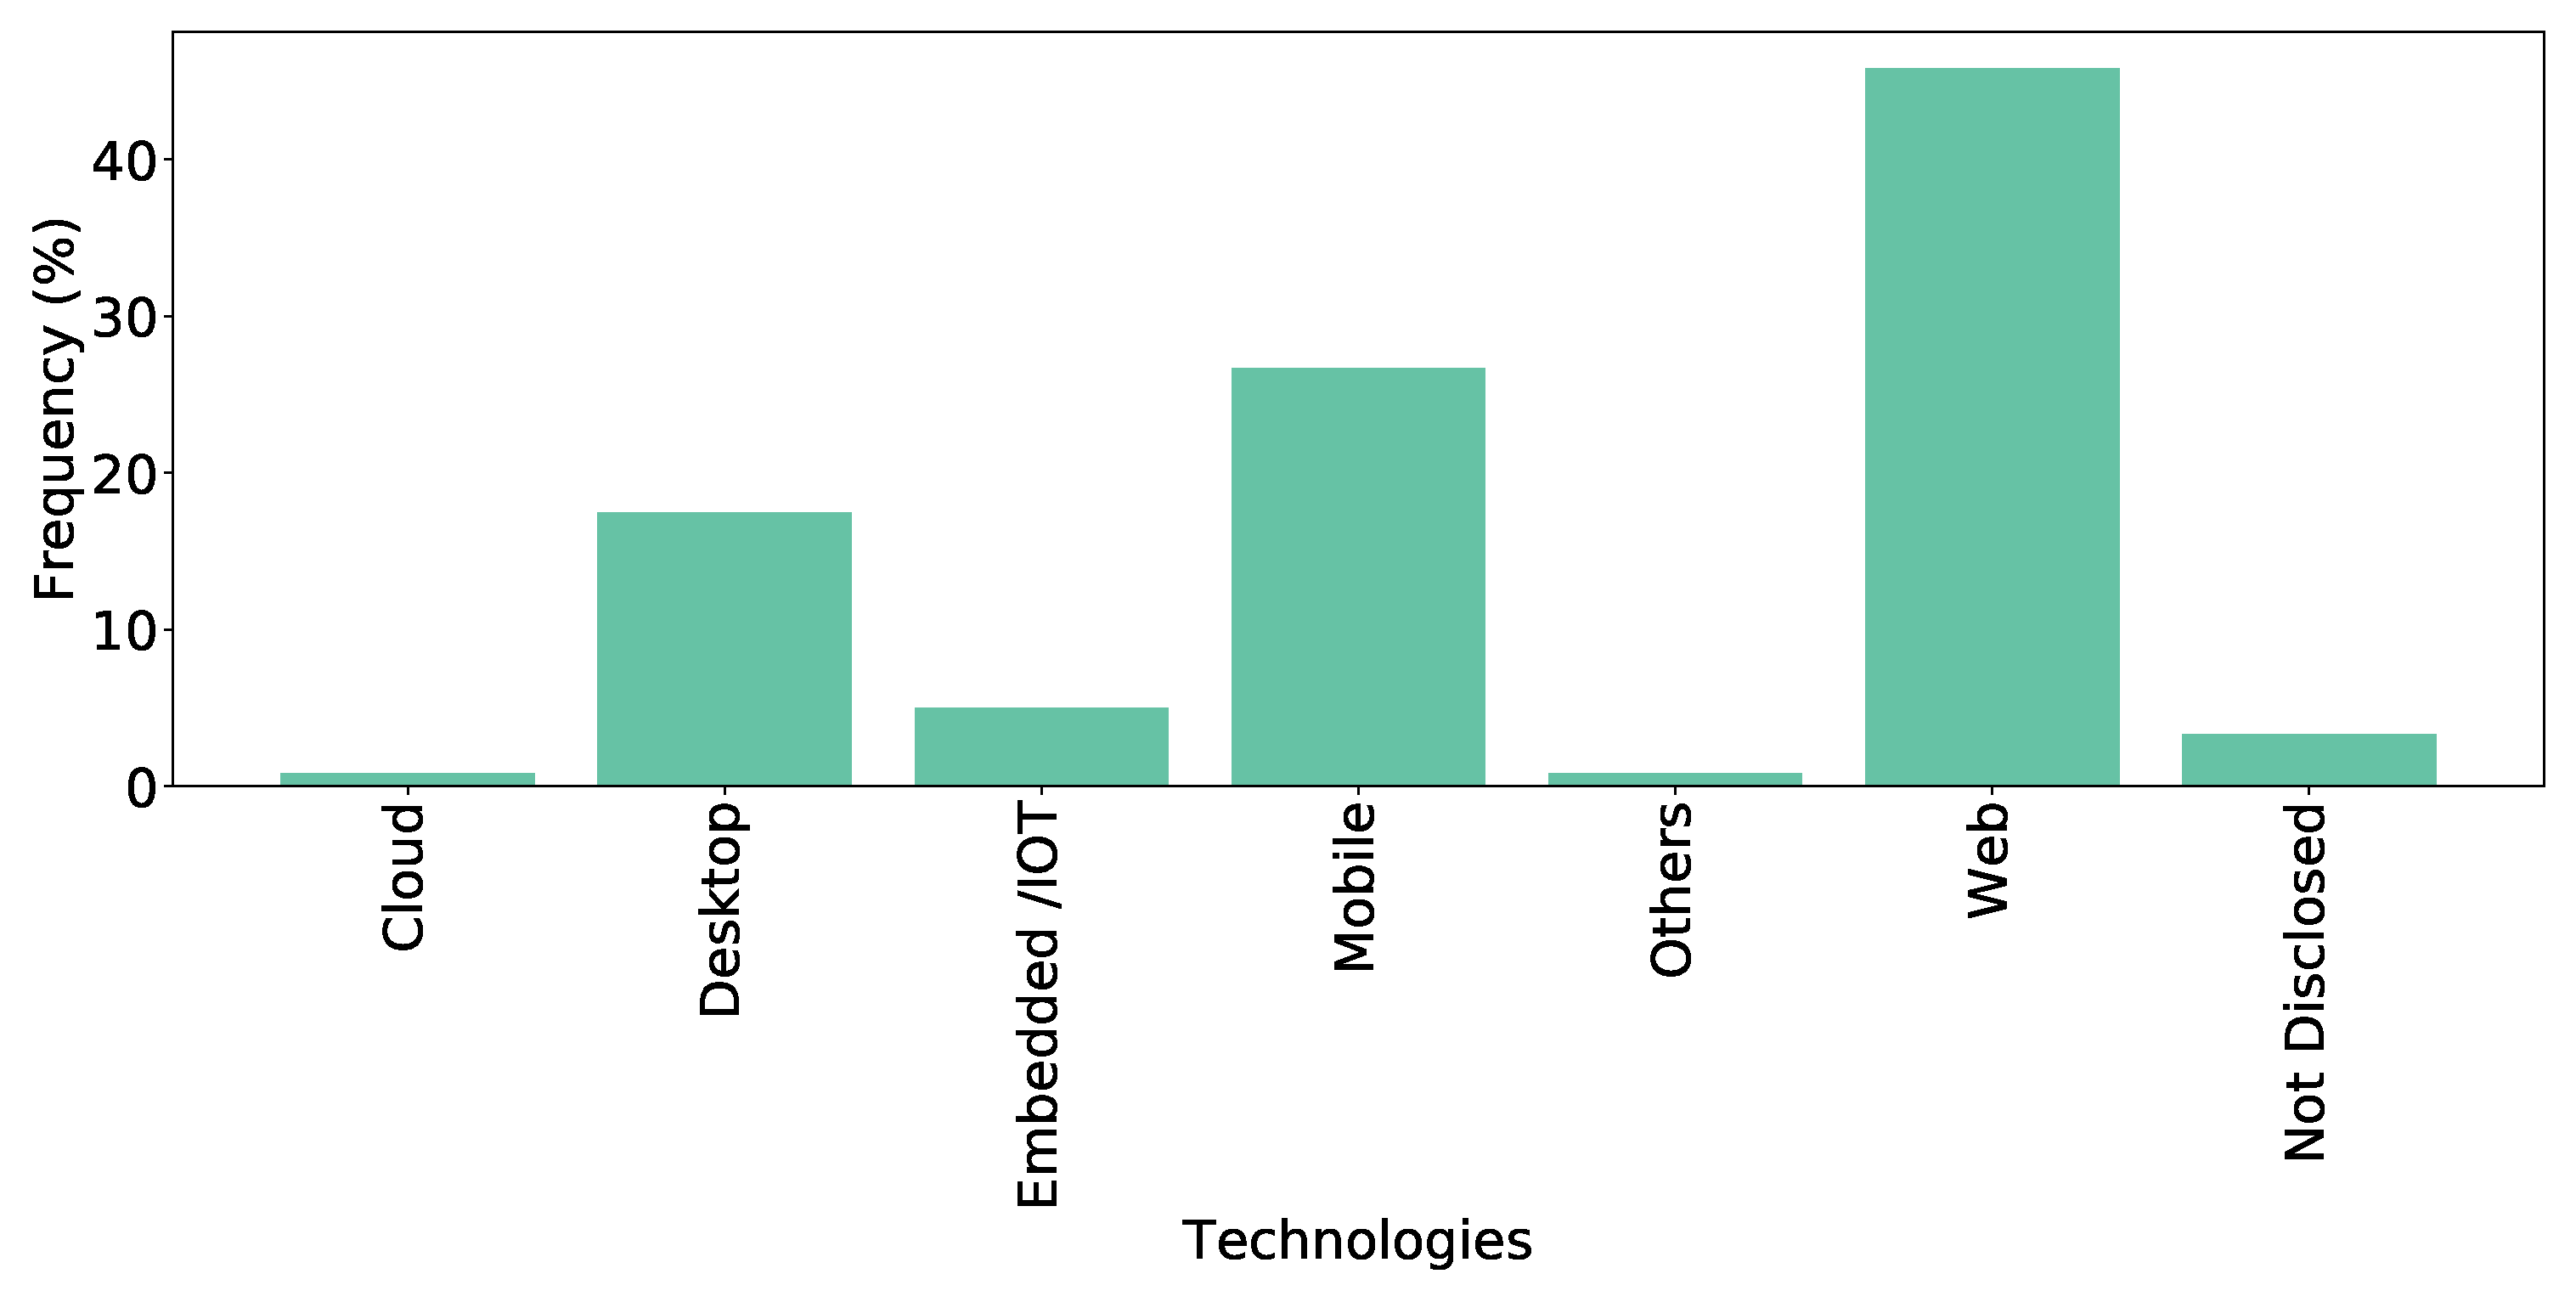
\includegraphics[width=0.8\textwidth]{Figures/Respondents_Technologies}
  \caption{Technology Platforms}
  \label{fig:platforms}
\end{figure}

\subsubsection{Operating Systems}
Most of our respondent's used linux based operating system (40\%). The second best used operating system is windows (32.5\%).
\begin{figure}[]
\centering
  \includegraphics[width=0.8\textwidth]{Figures/Respondents_os}
  \caption{Operating Systems}
  \label{fig:os}
\end{figure}

\subsubsection{Programming Languages}
According to \cref{fig:languages}, around 28\% of our respondent's used Java and Javascript each. Other languages like php, python, c\# are also used which indicates that the software engineers are not inclined towards a single specific language.
\begin{figure}[]
\centering
  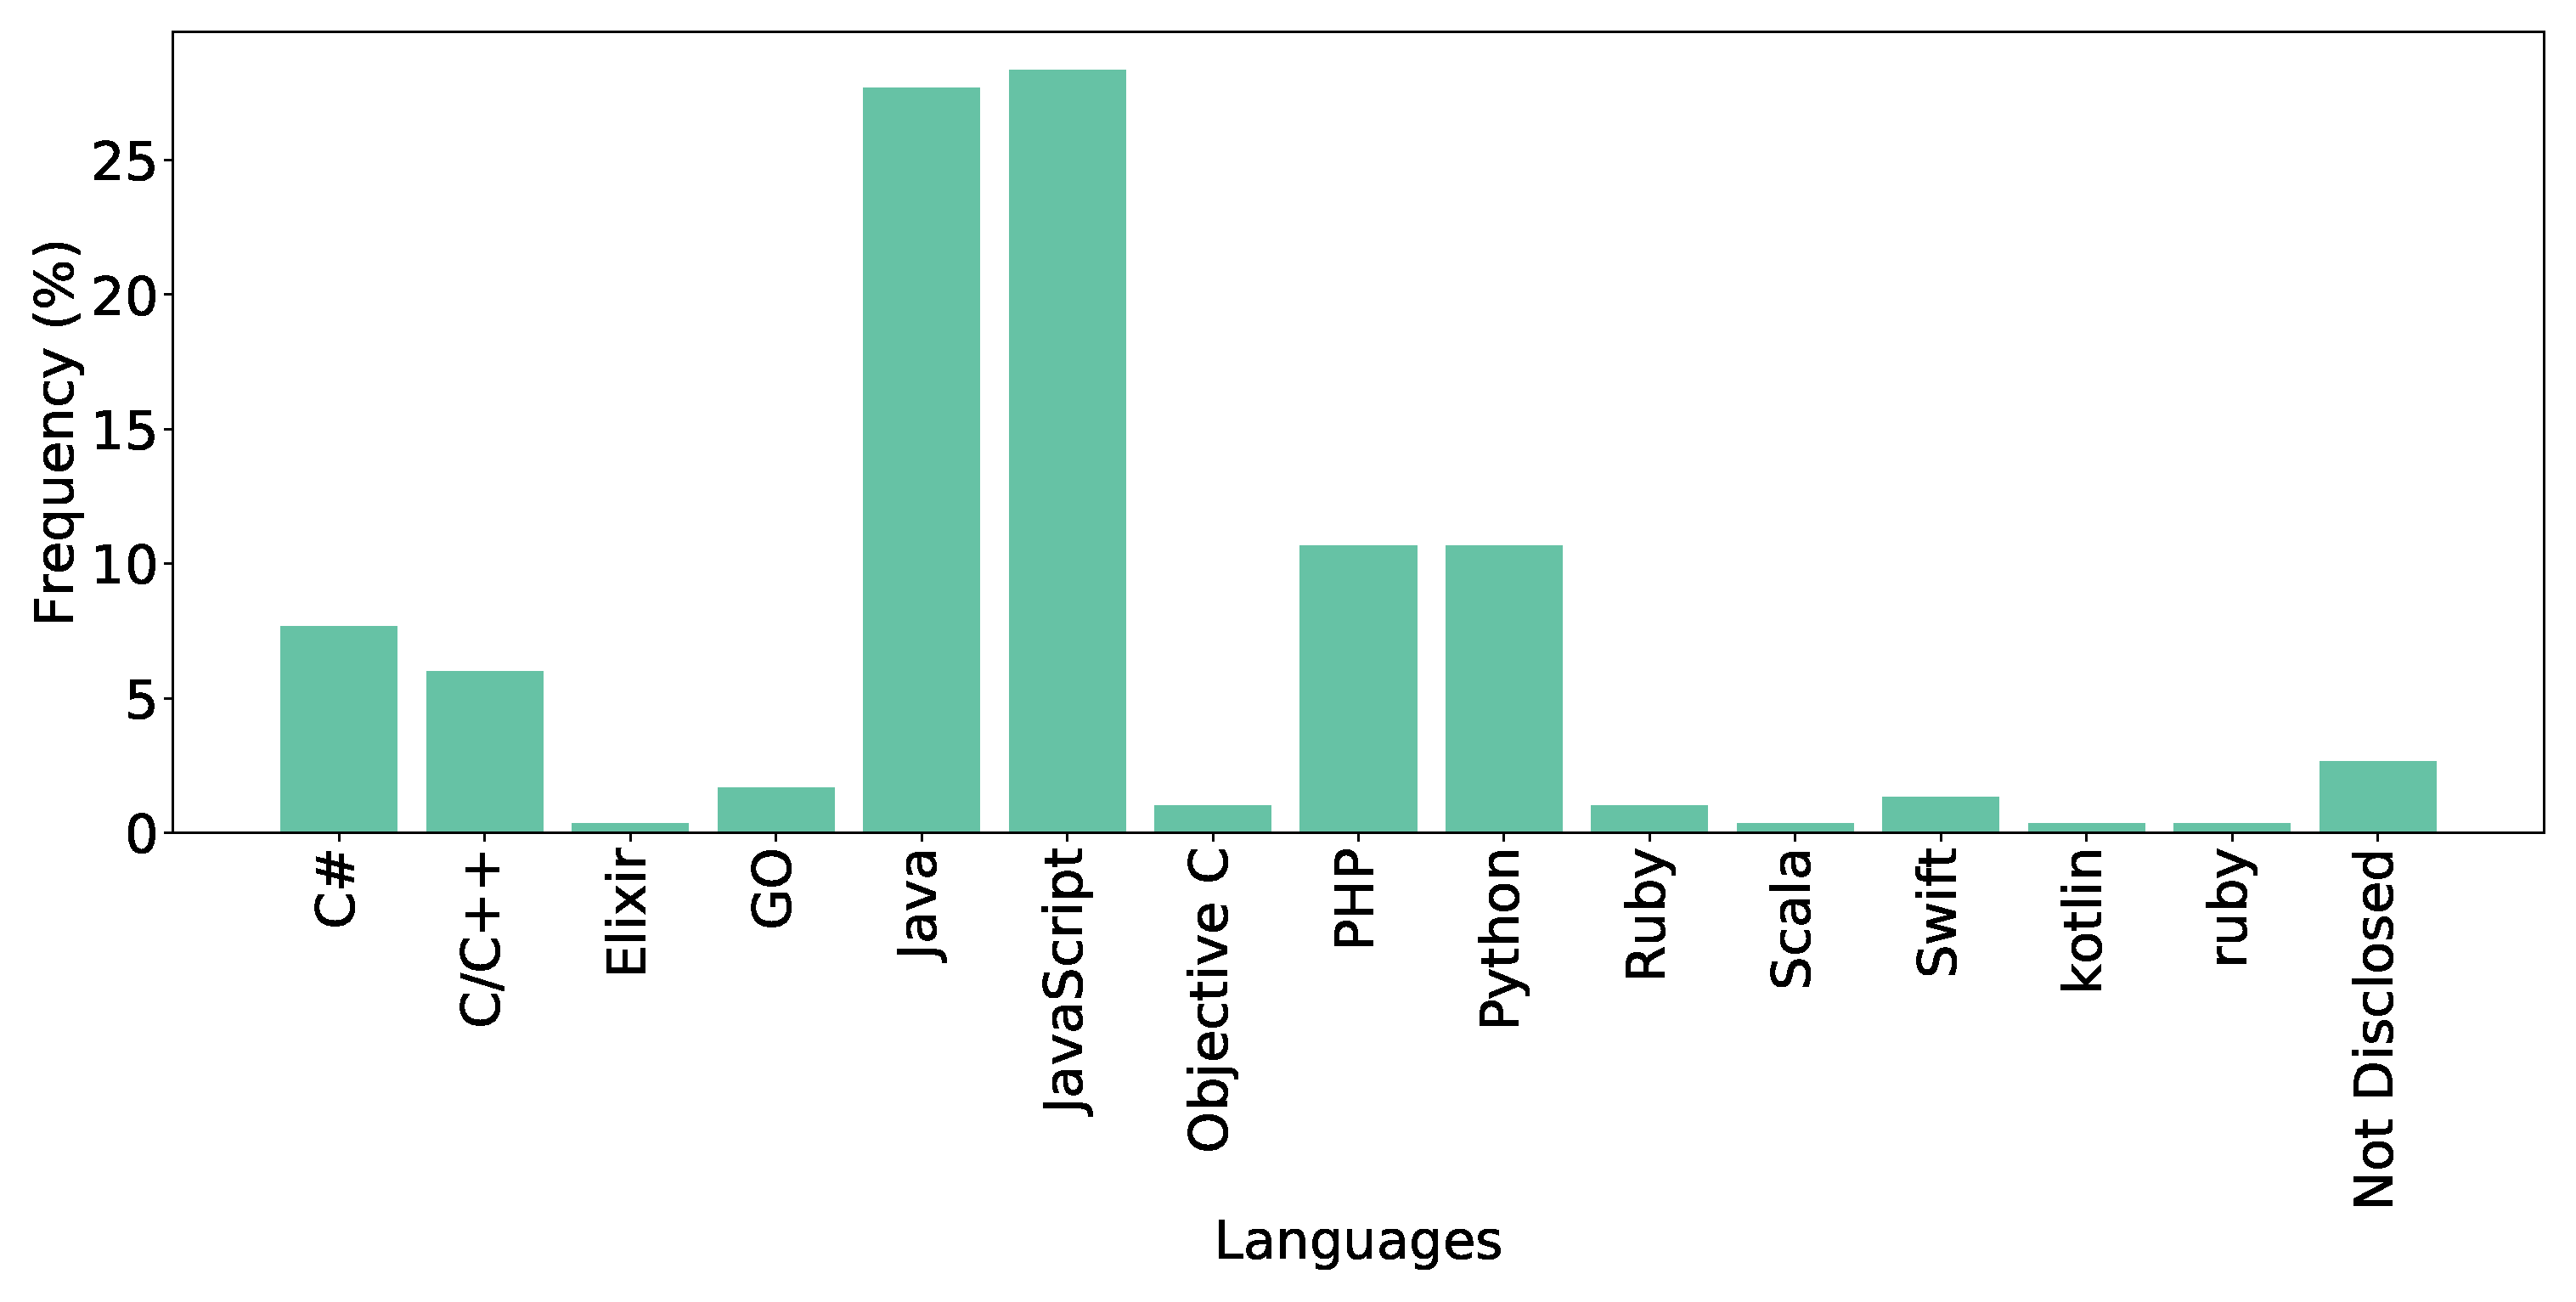
\includegraphics[width=0.8\textwidth]{Figures/Respondents_languages}
  \caption{Languages used in software development}
  \label{fig:languages}
\end{figure}

\subsubsection{Frameworks used in development}
As shown in \cref{fig:frameworks}, Spring boot (24\%) is the mostly used framework in the industry. ASP.NET, Django and Laravel are used in same proportion.
\begin{figure}[]
\centering
  \includegraphics[width=0.8\textwidth]{Figures/Respondents_frameworks}
  \caption{Frameworks}
  \label{fig:frameworks}
\end{figure}

\subsubsection{IDE's used by the respondent's}
According to \cref{fig:IDEs}, IntelliJ, a Java integrated development environment for developing computer software for enterprise, mobile, and web development used by most of the respondents (24\%). The other IDEs used in SE industries are: visual studio (20\%), Eclipse(15.6\%), PyCharm(11.2\%), NetBeans(7.3\%), Android Studio(4.4\%).
\begin{figure}[]
\centering
  \includegraphics[width=0.8\textwidth]{Figures/Respondents_IDEs}
  \caption{IDE's}
  \label{fig:IDEs}
\end{figure}
